% !TeX spellcheck = de_DE
\documentclass{uebung_cs}
\usepackage{algo123}
\uebung{8}{}{}
\blattname{Disjunkte Mengen, Union-Find}

%%%%%%%%%%%%%%%%%%%%%%%%%%%%%%%%%%%%%%%%%%%%%%%%%%%%%%%%%%%%%%%%%%%%%%%%%%%%

\newboolean{programming}
\setboolean{programming}{false}

%%%%%%%%%%%%%%%%%%%%%%%%%%%%%%%%%%%%%%%%%%%%%%%%%%%%%%%%%%%%%%%%%%%%%%%%%%%%
% Makros für noch nicht übersetzte Begrifflichkeiten
\newcommand{\qfind}{\textit{\textbf{Quick Find}}}
\newcommand{\qunion}{\textit{\textbf{Quick Union}}}
\newcommand{\wqunion}{\textit{\textbf{Weighted Quick Union}}}
\newcommand{\pathcomp}{\textit{\textbf{Pfadverkürzung}}}


\begin{document}
\textbf{Eigenständige Vorbereitung:}\\
Lies \emoji{book} CLRS Kapitel 21 ohne 21.4 (oder Algorithms 4ed. Kapitel 1.5) und schau dir das \emoji{television} Video der Woche an.

\textbf{Zeichenlegende:}
\legende{}

%  \schriftlich
%  \bestehen
%  \mittel
%  \note
%  \spass

\begin{aufgabe}[Union Find von Hand laufen lassen]\label{tue-first}
	Betrachte die folgende Sequenz von Operationen:
	\texttt{Init(7)}, \texttt{Union(3,4)}, \texttt{Union(5,0)}, \texttt{Union(4,5)}, \texttt{Union(4,3)}, \texttt{Union(0,1)}, \texttt{Union(2,6)}, \texttt{Union(0,4)} und \texttt{Union(6,0)}.
	\begin{enumerate}
		\item (\warmup) Führe die Sequenz mittels \qfind{} von Hand durch.
		Zeige, wie die Inhalte des Feldes \texttt{id} nach jedem Schritt aussehen.
		Die Operation \texttt{Union($i,j$)} verändert \texttt{id} hierbei immer für die Menge, die durch $i$ gegeben ist.
		\item (\warmup) Führe die Sequenz mittels \qunion{} von Hand durch.
		Zeige, wie der Baum nach jedem Schritt aussieht.
		Die Operation \texttt{Union($i,j$)} setzt hierbei immer die Wurzel von Baum von $i$ als ein Kind der Wurzel des Baumes von $j$.
		\item Führe die Sequenz mittels \wqunion{} von Hand durch.
		Zeige, wie der Baum nach jedem Schritt aussieht.
		Die Operation \texttt{Union($i,j$)} setzt hierbei immer die Wurzel von Baum von $i$ als ein Kind der Wurzel des Baumes von $j$, wenn die Größe der beiden Bäume gleich ist.
		\item Zeige das Resultat der \pathcomp{} nach einer Operation \texttt{Find($x$)} in einem der Bäume aus den Beispielen in a) und b), wobei $x$ einmal ein Blatt sein soll, einmal ein interner Knoten von Tiefe~$1$, und einmal ein interner Knoten mit Höhe~$1$.
		\item Gib eine Sequenz von Operationen an, die in einem Baum maximaler Tiefe resultieren, wenn die abstrakte Datenstruktur durch \qunion{} implementiert ist.
		\item Gib eine Sequenz von Operationen an, die in einem Baum maximaler Tiefe resultieren, wenn die abstrakte Datenstruktur durch \wqunion{} implementiert ist.
		\item Schreibe den Pseudo-Code für~\pathcomp{}. \emph{Hinweis: Durchlaufe den Pfad zweimal.}
	\end{enumerate}
\end{aufgabe}

\begin{aufgabe}[Alternative zum \qfind{} Algorithmus]
	Eine Kommilitonin stellt die folgende, intuitive Variante von \qfind{} \texttt{Union} vor.
	Funktioniert sie?
	\begin{algorithmic}
		\Procedure{Union}{$i, j$}
		\If{\Call{Find}{$i$} $\neq$ \Call{Find}{$j$}}
			\ForAll{$k \in \{0,\dots,n-1\}$}
				\If{\texttt{id[$k$] == id[$i$]}}
					\State \texttt{id[$k$] = id[$j$]}
				\EndIf
			\EndFor
		\EndIf
		\EndProcedure
	\end{algorithmic}
\end{aufgabe}

\begin{aufgabe}[Dynamische Zusammenhangskomponente und Suche in Graphen]\mbox{}\\
	Mit Tiefen- und Breitensuche können wir die Zusammenhangskomponenten eines Graphen finden.
	Entwirf einen einfache Implementierung der abstrakten Datenstruktur für den dynamischen Zusammenhang (mit den Operationen \textsc{Init}, \textsc{Connected}, \textsc{Insert}) mittels Suche in Graphen und vergleiche die Komplexität deiner Lösung mit der auf Union-Find basierenden Lösungen.
\end{aufgabe}


\begin{aufgabe}[Implementierung von Union-Find, alleine probieren]
	Wir wollen Datenstrukturen für Union-Find (mit den Operationen \texttt{Init}, \texttt{Union} und \texttt{Find}) in einer beliebigen Programmiersprache implementieren.
	\begin{enumerate}
		\item Implementiere \qunion{}.
		\item Erweitere deine Implementierung mit \wqunion{}.
		\item Erweitere deine Implementierung mit \pathcomp{}.
	\end{enumerate}
\end{aufgabe}

\begin{aufgabe}[Zombieinvasion, \hard]
	Der erkenntnisgierige Prof.~Dr.~Regloh hat bei unethischen Zombieduellexperimenten versehentlich einige Zombies entkommen lassen und damit die postapokalyptische Zukunft eingeläutet.
	Du hast dich mit einer kleinen Gruppe an Überlebenden in einem kleinen Gebäude verbarrikadiert.
	Das Einzige, das zwischen euch und einer brutalen und hungrigen Horde Zombies steht, ist eine starke Befestigung. Die Befestigung besteht aus einem $k\times k$ Gitter von Wänden, hier illustriert durch ein $6\times 6$ Gitter von Wänden (\emph{graue Rechtecke}):

	\begin{center}
		\newcommand{\wallAt}[2]{
			% draws 1x0.6 wall at (#1,#2)
			\draw[fill=black!25,draw=none] (#1-0.45,#2*0.7+0.3) rectangle (#1+0.45,#2*0.7-0.3);
		}
		\begin{tikzpicture}
			% draw each layer
			\foreach \x in {0,1,2,4}{
				\wallAt{\x}{0}
			}
			\foreach \x in {0,2,4,5}{
				\wallAt{\x}{1}
			}
			\foreach \x in {1,2,3,4,5}{
				\wallAt{\x}{2}
			}
			\foreach \x in {2,5}{
				\wallAt{\x}{3}
			}
			\foreach \x in {1,2,4,5}{
				\wallAt{\x}{4}
			}
			\foreach \x in {1,2,3,4,5}{
				\wallAt{\x}{5}
			}
			% draw delimiters
			\draw[line width=2pt] (-0.7,5*0.7 + 1) -- (-0.7,-1);
			\draw[line width=2pt] (5.7,5*0.7 + 1) -- (5.7,-1);
		\end{tikzpicture}
		\hspace{0.7cm}
		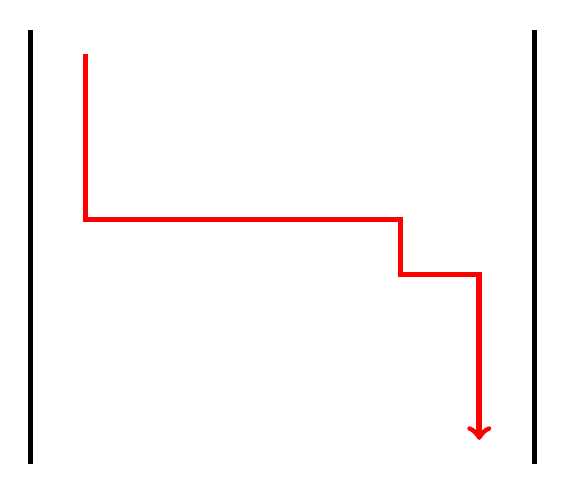
\begin{tikzpicture}
			% draw each layer
			\foreach \x in {0,1,2,4}{
				\wallAt{\x}{0}
			}
			\foreach \x in {2,4}{
				\wallAt{\x}{1}
			}
			\foreach \x in {1,2,3}{
				\wallAt{\x}{2}
			}
			\foreach \x in {5}{
				\wallAt{\x}{3}
			}
			\foreach \x in {1,2,5}{
				\wallAt{\x}{4}
			}
			\foreach \x in {1,3,4}{
				\wallAt{\x}{5}
			}
			% draw delimiters
			\draw[line width=2pt] (-0.7,5*0.7 + 1) -- (-0.7,-1);
			\draw[line width=2pt] (5.7,5*0.7 + 1) -- (5.7,-1);
			% zombie path
			\draw[->, line width=2pt, red] (0, 6*0.7) -- (0,3*0.7) -- (4,3*0.7) -- (4,2*0.7) -- (5,2*0.7) -- (5,-0.7); 
		\end{tikzpicture}
	\end{center}
	Oberhalb des Gitters warten die Zombies, während deine Gruppe und du unterhalb sind.
	Unglücklicherweise sind die Wände alt und spröde, und stürzen regelmäßig ein.
	Sobald ein Pfad von ganz oben nach ganz unten verläuft, kommen die Zombies durch.
	Um eure Evakuierung vorzubereiten, willst du durchgehend überwachen, ob es derzeit einen Pfad durch die Befestigung gibt.
	Entwirf eine Datenstruktur, die effizient den Überblick behält, während die Wände (Zellen des Gitters) eine nach der anderen einstürzen.
\end{aufgabe}

\begin{aufgabe}[Rekursive \pathcomp, \hard]
	Entwirf eine rekursive Variante von \pathcomp{} in Pseudo-Code.
\end{aufgabe}

\begin{aufgabe}[Union-Find mit verketteten Listen und Gewichtungen]
	Wir wollen eine Variante von \qfind{} mittels verketteten Listen auf die folgende Art und Weise implementieren.
	Jede Menge wird durch eine einfach verkettete Liste repräsentiert.
	Der Repräsentant jeder Menge ist das erste Element der jeweiligen Liste und jedes Element der Liste hat einen Zeiger auf den Repräsentanten.
	Des Weiteren haben wir einen Zeiger \texttt{tail} auf das letzte Element der Liste.
	Zum Beispiel könnte die Datenstruktur für die Menge $\{1,4,7,8,14\}$ mit Repräsentant $7$ wie folgt aussehen:
	\begin{center}
		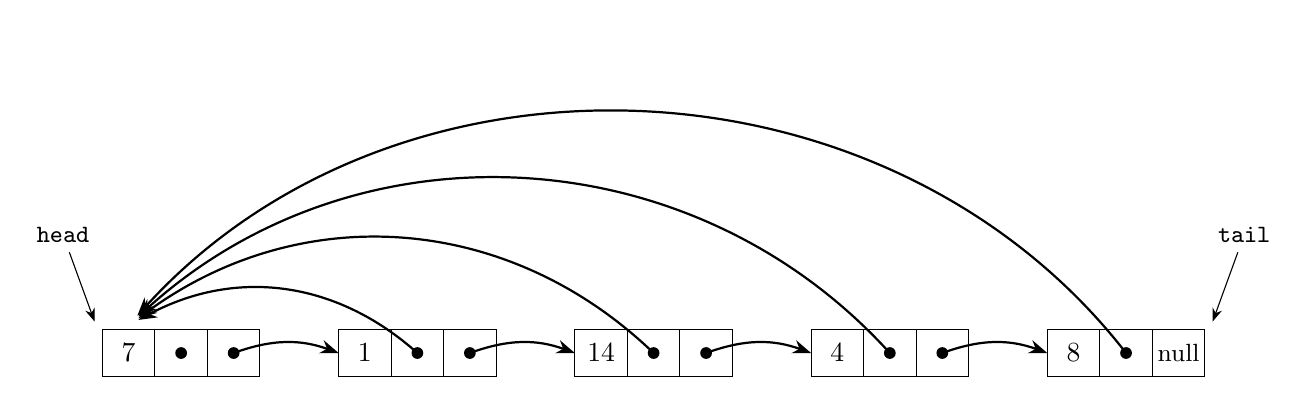
\begin{tikzpicture}
			\usetikzlibrary{arrows.meta}
			\newcommand{\listElem}[4]{  
				% draws list elements 
				% args: 
				%     "rank" (ordered left to right)
				%     label
				%     fill color for base circle of next pointer
				%     text at next pointer slot
				\draw (#1*3, 0.3) rectangle (#1*3 + 2,-0.3);
				\draw (#1*3 + 2/3, 0.3) -- (#1*3 + 2/3, -0.3);
				\draw (#1*3 + 4/3, 0.3) -- (#1*3 + 4/3, -0.3);
				\node (val_#2) at (#1*3 + 1/3, 0) {#2};
				\node (top_#2) at (#1*3 + 1/3, 0.35) {};
				\node (left_#2) at (#1*3, 0) {};
				\node[fill=black, circle, inner sep=1.5pt] (repr_#2) at (#1*3 + 1, 0) {};
				\node[fill=#3, circle, inner sep=1.5pt] (nxt_#2) at (#1*3 + 5/3, 0) {};
				\node () at (nxt_#2) {\small #4};
			}
			\newcommand{\listReprPtr}[3]{
				% args:
				%     from label
				%     to label
				%     bend angle
				\draw[-Stealth, thick] (repr_#1.center) to [bend right=#3] (top_#2);
			}
			\newcommand{\listNxtPtr}[3]{
				% args:
				%     from label
				%     to label
				%     bend angle
				\draw[-Stealth, thick] (nxt_#1.center) to [bend left=#3] (left_#2.center);
			}
			% wrappers
			\newcommand{\regularListElem}[2]{ \listElem{#1}{#2}{black}{} }
			\newcommand{\tailListElem}[2]{ \listElem{#1}{#2}{white}{null} }
			%
			% draw the list
			% elements of the list
			\regularListElem{0}{7}
			\regularListElem{1}{1}
			\regularListElem{2}{14}
			\regularListElem{3}{4}
			\tailListElem{4}{8}
			% representative pointers
			% aufsteigende grade sorgen dafür, dass die pfeilspitzen nicht
			% alle exakt im selben punkt landen
			\listReprPtr{1}{7}{35}
			\listReprPtr{14}{7}{40}
			\listReprPtr{4}{7}{45}
			\listReprPtr{8}{7}{50}
			% next pointers
			\listNxtPtr{7}{1}{20}
			\listNxtPtr{1}{14}{20}
			\listNxtPtr{14}{4}{20}
			\listNxtPtr{4}{8}{20}
			% head ptr, tail ptr
			\node (headptr) at (-0.5, 1.5) {\texttt{\small head}};
			\node (tailptr) at (14.5, 1.5) {\texttt{\small tail}};
			\draw[-Stealth] (headptr) -- (-0.1, 0.4);
			\draw[-Stealth] (tailptr) -- (14.1, 0.4);
		\end{tikzpicture}
	\end{center}
	\begin{enumerate}
		\item Zeige wie man mit dieser Darstellung der Mengen die Operationen \texttt{Init($n$)} in Zeit $O(n)$, \texttt{Find($i$)} in Zeit $O(1)$ und \texttt{Union($i,j$)} in Zeit $O(|S(i)|)$ implementieren kann, wobei $S(i)$ diejenige Menge ist, die $i$ enthält.
		\item\label{min} Zeige, wie man die Lösung erweitern kann, sodass \texttt{Init} und \texttt{Find} dieselbe Zeitkomplexität wie zuvor haben, aber \texttt{Union($i,j$)} nun nur Zeit $O(\min(|S(i)|, |S(j)|))$ benötigt.
			\textit{Hinweis: Speichere ein paar Zusatzinformationen.}
		\item (\hard) Zeige, dass für die Lösung aus \ref{min} jede Sequenz von $p$ \texttt{Find} und $m$ \texttt{Union} Operationen auf $n$ Elementen eine Laufzeit von $O(p + m\log n)$ hat.
		Zu Beginn der Sequenz sind alle Mengen einelementig.
	\end{enumerate}
\end{aufgabe}

\begin{aufgabe}[Union Find Move \schriftlich]
  Entwickle eine \textbf{möglichst effiziente} Implementierung der folgenden abstrakten Datenstruktur:
  Verwalte eine Familie von disjunkten Mengen, anfangs die einelementigen Mengen
  \[ \{0\},\{1\}, \ldots,\{n-1\}\,,\]
  unter den folgenden Operationen:
  \begin{description}
   \item[0 (\enquote{query})]
      Die \emph{query} Operation nimmt zwei Argumente $s$ und $t$, und ermittelt, ob $s$ und $t$ zur selben Menge gehören.
      Das heißt, wenn $s\in S$ and $t\in T$, dann gibt die Operation \texttt{1} aus falls $S=T$ und \texttt{0} wenn $S\neq T$.
    \item[1 (\enquote{union})]
    Die \emph{union} Operation nimmt zwei Argumente $s$ und $t$, und erzeugt die Vereinigung der beiden Mengen, die $s$ und $t$ enthalten.
    Das heißt, wenn $s\in S$ und $t\in T$ mit $S\neq T$, dann sollen $S$ und $T$ aus der Familie entfernt und durch die Menge $S\cup T$ ersetzt werden.
      (Wenn $S=T$, dann passiert nichts.)
    \item[2 (\enquote{move})]
      Die \emph{move} Operation nimmt zwei Argumente $s$ und $t$, und verschiebt das Element $s$ in die Menge, die $t$ enthält.
      Das heißt, wenn $s\in S$ und $t\in T$ mit $S\neq T$, dann sollen $S$ und $T$ aus der Familie entfernt werden und stattdessen die Mengen $S-\{s\}$ (falls diese nichtleer ist)  und $T\cup\{s\}$ zur Familie hinzugefügt werden.
      (Wenn $S= T$, dann passiert nichts.)
  \end{description}
  Diese Operationen erhalten die Invariante, dass die Mengen in der Familie disjunkt sind.
  
  \begin{enumerate}
    \item\label{describe} Beschreibe deine Datenstruktur und analysiere sie
    \item\label{implement} Implementiere und teste deine Datenstruktur gemäß der Anforderungen in Abschnitt~\ref{implementierung}.
  \end{enumerate}

  \textbf{Hinweise zur Abgabe.}
  %Mindestens~\ref{describe} muss bearbeitet werden.
  Die Union-Find Datenstrukturen aus der Vorlesung reichen hier nicht aus, sondern müssen modifiziert werden, daher ist eine klare und anschauliche Beschreibung der Idee besonders wichtig. Kleine Bildchen wären nützlich, um den Zustand deiner Datenstruktur zu verstehen.
  Erwartet werden ansonsten wie üblich die grobe Idee, Pseudocode oder echter Code, Korrektheitsbeweis, Laufzeitanalyse.

  \appendix
  \section{Implementierung}\label{implementierung}
  Für die Implementierung soll folgendes Ein- und Ausgabeverhalten unterstützt werden.
  \subsection*{Eingabe}
  
  Die Eingabe startet mit zwei natürlichen Zahlen $n$ und $m$ in der ersten Zeile.
  Die Zahl $n$ ist die Anzahl an einelementigen Mengen zu Beginn.
  Dann folgen $m$ Zeilen der Form
  \enquote{\texttt{0} $s$ $t$} (für \emph{query}) oder \enquote{\texttt{1} $s$ $t$} (für \emph{union}) oder \enquote{\texttt{2} $s$ $t$} (für \emph{move}).
  Du kannst $0\leq s< n$ und $0\leq t< n$ annehmen.

  \subsection*{Ausgabe}
  
  Für jede \emph{query} Operation wird wie oben beschrieben eine Zeile mit \texttt{1} oder \texttt{0} ausgegeben.
  
  \subsection*{Beispiel}
  \begin{tabular}{ll}
  \texttt{example.in}& Zustand der Datenstruktur nach der Operation\\
    \texttt{4 9}   & $\{0\}, \{1\}, \{2\},\{3\}$\\
    \texttt{0 0 1} \\
    \texttt{1 0 1} & $\{0, 1\}, \{2\},\{3\}$ \\
    \texttt{0 0 1} &\\
    \texttt{1 1 2} & $\{0, 1, 2\},\{3\}$ \\
    \texttt{0 1 2} &\\
    \texttt{0 0 3} &\\
    \texttt{2 2 3}   & $\{0, 1\}, \{2,3\}$ \\
    \texttt{0 0 1} &\\
    \texttt{0 1 2} &
  \end{tabular}

  \noindent
  \begin{verbatim}
example.ans
0
1
1
0
1
0
  \end{verbatim}

  \subsection*{Mehr Tests}
  Hier gibt es größere Tests:\\
  \small\url{https://tcs.uni-frankfurt.de/teaching/summer21/algo1/unionfindmove-tests-v2.zip}

  Die darin enthaltene Datei \verb|032-huge.in| sollte gelöst werden.
  Ein effizienter Algorithmus braucht auf einem handelsüblichen Laptop nicht lange:
  \begin{verbatim}
$ time python oursolution.py < 032-huge.in > /dev/null

________________________________________________________
Executed in    8.85 secs    fish           external
   usr time    8.79 secs  822.00 micros    8.79 secs
   sys time    0.06 secs  309.00 micros    0.06 secs
  \end{verbatim}
  Liefern Sie die SHA-1 Summe von \verb|032-huge.ans|.

\end{aufgabe}

\end{document}
